\documentclass[aspectratio=169]{beamer}

% Minimal theme
\usetheme{default}
\usecolortheme{dove}

% Remove navigation symbols
\setbeamertemplate{navigation symbols}{}
\setbeamertemplate{footline}{%
  \hfill{\large\insertframenumber\,/\,\inserttotalframenumber}\hspace{0.8em}\vspace{0.5em}%
}

% Colors
\definecolor{popblue}{RGB}{52, 101, 164}
\definecolor{sampred}{RGB}{204, 0, 0}
\definecolor{paramgreen}{RGB}{0, 140, 70}
\definecolor{lightbg}{RGB}{245, 245, 250}
\definecolor{warnred}{RGB}{180, 40, 40}
\definecolor{orange1}{RGB}{220, 120, 0}
\definecolor{violet1}{RGB}{120, 50, 160}

\setbeamercolor{frametitle}{fg=popblue}
\setbeamercolor{title}{fg=popblue}

% Packages
\usepackage{pgfplots}
\usepackage{tikz}
\usetikzlibrary{shapes, arrows.meta, positioning, calc, decorations.pathreplacing, patterns, fit}
\pgfplotsset{compat=1.18}
\usepackage{amsmath, amssymb}
\usepackage{array}
\usepackage{fontenc}

\title{Hallucination \& Grounding}
\subtitle{Detection $\cdot$ Mitigation $\cdot$ Calibration $\cdot$ Attribution}
\date{}

\begin{document}

% ============================================================
% TITLE
% ============================================================
\begin{frame}
\titlepage
\end{frame}

% ============================================================
% WHAT IS HALLUCINATION?
% ============================================================
\begin{frame}
\frametitle{What is hallucination?}

\begin{center}
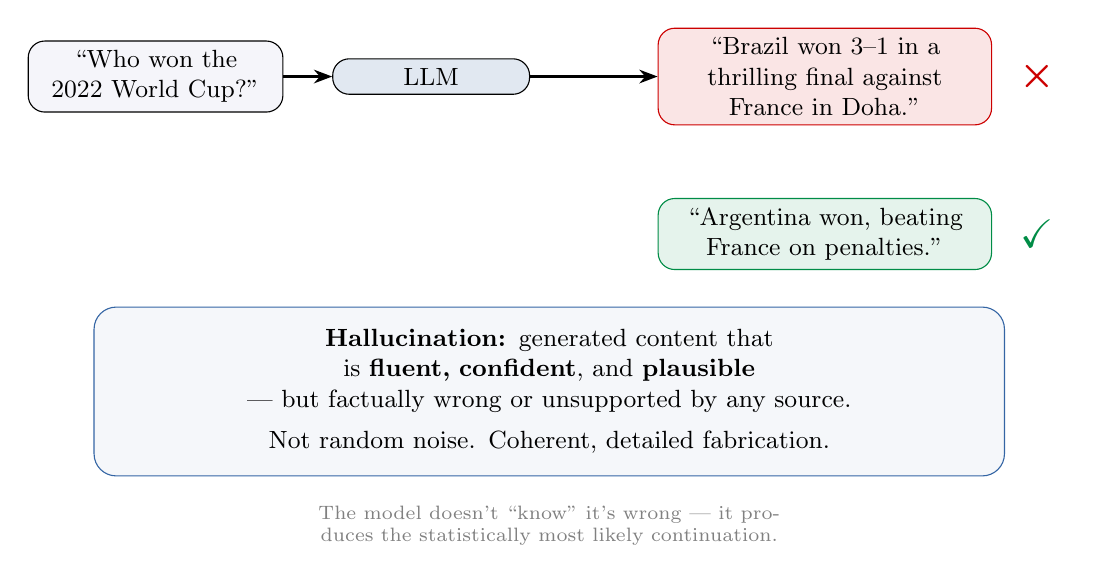
\begin{tikzpicture}
  % Prompt
  \node[draw, rounded corners=6pt, fill=lightbg, minimum width=3cm, font=\small, text width=3cm, align=center] (prompt) at (-5, 2.5) {``Who won the\\2022 World Cup?''};

  % Model
  \node[draw, rounded corners=6pt, fill=popblue!15, minimum width=2.5cm, font=\small] (model) at (-1.5, 2.5) {LLM};
  \draw[-Stealth, thick] (prompt) -- (model);

  % Hallucinated answer
  \node[draw=sampred, rounded corners=6pt, fill=sampred!10, minimum width=3.5cm, font=\small, text width=4cm, align=center] (bad) at (3.5, 2.5) {``Brazil won 3--1 in a\\thrilling final against\\France in Doha.''};
  \draw[-Stealth, thick] (model) -- (bad);
  \node[font=\Large, text=sampred] at (6.2, 2.5) {$\boldsymbol{\times}$};

  % What it should say
  \node[draw=paramgreen, rounded corners=6pt, fill=paramgreen!10, font=\small, text width=4cm, align=center] (good) at (3.5, 0.5) {``Argentina won, beating\\France on penalties.''};
  \node[font=\Large, text=paramgreen] at (6.2, 0.5) {$\checkmark$};

  % Definition
  \node[draw=popblue, fill=popblue!5, rounded corners=8pt, text width=11cm, align=center, inner sep=8pt, font=\small] at (0, -1.5) {
    \textbf{Hallucination:} generated content that is \textbf{fluent, confident}, and \textbf{plausible}\\
    --- but factually wrong or unsupported by any source.\\[4pt]
    Not random noise. Coherent, detailed fabrication.
  };

  % Key point
  \node[font=\scriptsize, text=gray, text width=11cm, align=center] at (0, -3.2) {
    The model doesn't ``know'' it's wrong --- it produces the statistically most likely continuation.
  };
\end{tikzpicture}
\end{center}
\end{frame}

% ============================================================
% TAXONOMY
% ============================================================
\begin{frame}
\frametitle{Taxonomy of hallucinations}

\begin{center}
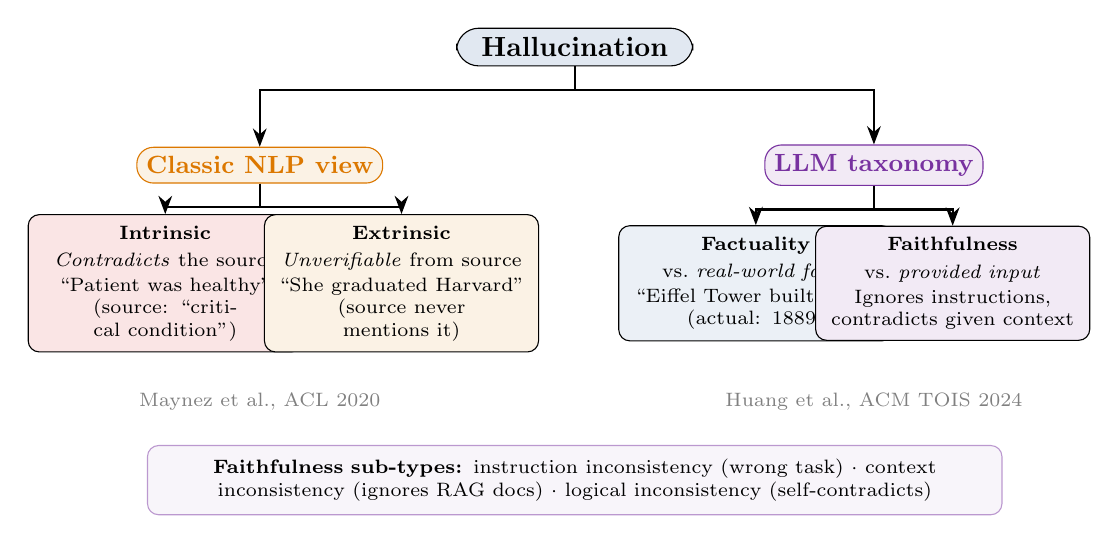
\begin{tikzpicture}
  % Root
  \node[draw, rounded corners=8pt, fill=popblue!15, font=\normalsize\bfseries, minimum width=3cm] (root) at (0, 3) {Hallucination};

  % Branch 1: Classic NLP
  \node[draw=orange1, fill=orange1!10, rounded corners=6pt, font=\small\bfseries, text=orange1, minimum width=2.5cm] (classic) at (-4, 1.5) {Classic NLP view};

  % Intrinsic / Extrinsic
  \node[draw, rounded corners=4pt, fill=sampred!10, font=\scriptsize, text width=3.2cm, align=center, inner sep=4pt] (intr) at (-5.2, 0) {
    \textbf{Intrinsic}\\[2pt]
    \emph{Contradicts} the source\\[1pt]
    ``Patient was healthy''\\(source: ``critical condition'')
  };
  \node[draw, rounded corners=4pt, fill=orange1!10, font=\scriptsize, text width=3.2cm, align=center, inner sep=4pt] (extr) at (-2.2, 0) {
    \textbf{Extrinsic}\\[2pt]
    \emph{Unverifiable} from source\\[1pt]
    ``She graduated Harvard''\\(source never mentions it)
  };

  \draw[-Stealth, thick] (root.south) -- ++(0,-0.3) -| (classic.north);
  \draw[-Stealth, thick] (classic.south) -- ++(0,-0.3) -| (intr.north);
  \draw[-Stealth, thick] (classic.south) -- ++(0,-0.3) -| (extr.north);

  % Branch 2: LLM taxonomy
  \node[draw=violet1, fill=violet1!10, rounded corners=6pt, font=\small\bfseries, text=violet1, minimum width=2.5cm] (llm) at (3.8, 1.5) {LLM taxonomy};

  % Factuality / Faithfulness
  \node[draw, rounded corners=4pt, fill=popblue!10, font=\scriptsize, text width=3.2cm, align=center, inner sep=4pt] (fact) at (2.3, 0) {
    \textbf{Factuality}\\[2pt]
    vs.\ \emph{real-world facts}\\[1pt]
    ``Eiffel Tower built 1920''\\(actual: 1889)
  };
  \node[draw, rounded corners=4pt, fill=violet1!10, font=\scriptsize, text width=3.2cm, align=center, inner sep=4pt] (faith) at (4.8, 0) {
    \textbf{Faithfulness}\\[2pt]
    vs.\ \emph{provided input}\\[1pt]
    Ignores instructions,\\contradicts given context
  };

  \draw[-Stealth, thick] (root.south) -- ++(0,-0.3) -| (llm.north);
  \draw[-Stealth, thick] (llm.south) -- ++(0,-0.3) -| (fact.north);
  \draw[-Stealth, thick] (llm.south) -- ++(0,-0.3) -| (faith.north);

  % References
  \node[font=\scriptsize, text=gray] at (-4, -1.5) {Maynez et al., ACL 2020};
  \node[font=\scriptsize, text=gray] at (3.8, -1.5) {Huang et al., ACM TOIS 2024};

  % Faithfulness sub-types
  \node[draw=violet1!50, fill=violet1!5, rounded corners=4pt, text width=10.5cm, align=center, inner sep=5pt, font=\scriptsize] at (0, -2.5) {
    \textbf{Faithfulness sub-types:} instruction inconsistency (wrong task) $\cdot$ context inconsistency (ignores RAG docs) $\cdot$ logical inconsistency (self-contradicts)
  };
\end{tikzpicture}
\end{center}
\end{frame}

% ============================================================
% TYPES OF HALLUCINATION
% ============================================================
\begin{frame}
\frametitle{Types of hallucination}

\vspace{-0.3cm}
\begin{center}
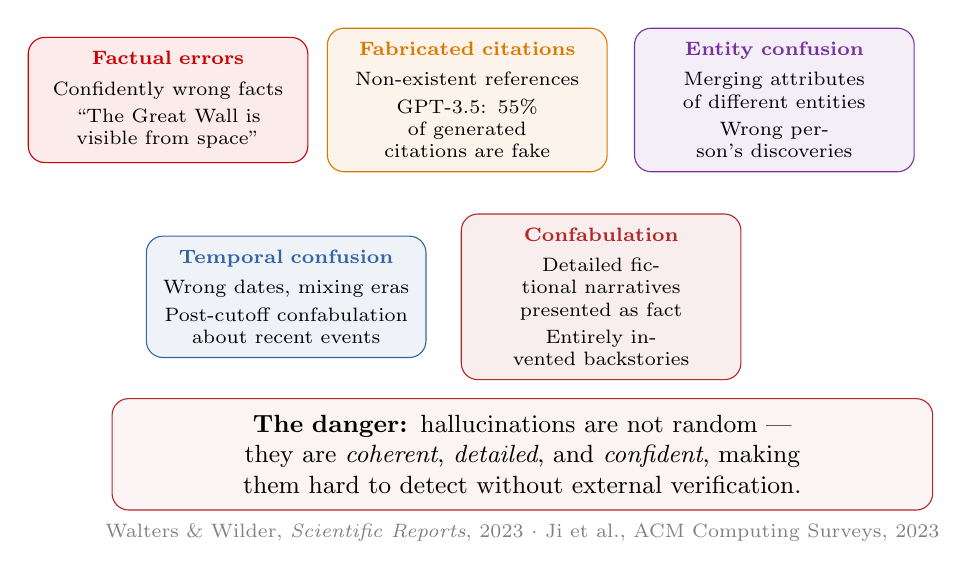
\begin{tikzpicture}
  % 5 cards in 2 rows
  % Row 1
  \node[draw=sampred, fill=sampred!8, rounded corners=6pt, text width=3.2cm, align=center, inner sep=5pt, font=\scriptsize] at (-4.5, 2) {
    \textbf{\textcolor{sampred}{Factual errors}}\\[3pt]
    Confidently wrong facts\\[2pt]
    ``The Great Wall is\\visible from space''
  };
  \node[draw=orange1, fill=orange1!8, rounded corners=6pt, text width=3.2cm, align=center, inner sep=5pt, font=\scriptsize] at (-0.7, 2) {
    \textbf{\textcolor{orange1}{Fabricated citations}}\\[3pt]
    Non-existent references\\[2pt]
    GPT-3.5: 55\% of generated\\citations are fake
  };
  \node[draw=violet1, fill=violet1!8, rounded corners=6pt, text width=3.2cm, align=center, inner sep=5pt, font=\scriptsize] at (3.2, 2) {
    \textbf{\textcolor{violet1}{Entity confusion}}\\[3pt]
    Merging attributes\\of different entities\\[2pt]
    Wrong person's discoveries
  };

  % Row 2
  \node[draw=popblue, fill=popblue!8, rounded corners=6pt, text width=3.2cm, align=center, inner sep=5pt, font=\scriptsize] at (-3, -0.5) {
    \textbf{\textcolor{popblue}{Temporal confusion}}\\[3pt]
    Wrong dates, mixing eras\\[2pt]
    Post-cutoff confabulation\\about recent events
  };
  \node[draw=warnred, fill=warnred!8, rounded corners=6pt, text width=3.2cm, align=center, inner sep=5pt, font=\scriptsize] at (1, -0.5) {
    \textbf{\textcolor{warnred}{Confabulation}}\\[3pt]
    Detailed fictional narratives\\presented as fact\\[2pt]
    Entirely invented backstories
  };

  % The danger
  \node[draw=warnred, fill=warnred!5, rounded corners=6pt, text width=10cm, align=center, inner sep=6pt, font=\small] at (0, -2.5) {
    \textbf{The danger:} hallucinations are not random --- they are \emph{coherent}, \emph{detailed}, and
    \emph{confident}, making them hard to detect without external verification.
  };

  % Reference
  \node[font=\scriptsize, text=gray] at (0, -3.5) {Walters \& Wilder, \emph{Scientific Reports}, 2023 $\cdot$ Ji et al., ACM Computing Surveys, 2023};
\end{tikzpicture}
\end{center}
\end{frame}

% ============================================================
% WHY — TRAINING & ARCHITECTURE
% ============================================================
\begin{frame}
\frametitle{Why LLMs hallucinate --- training \& architecture}

\begin{center}
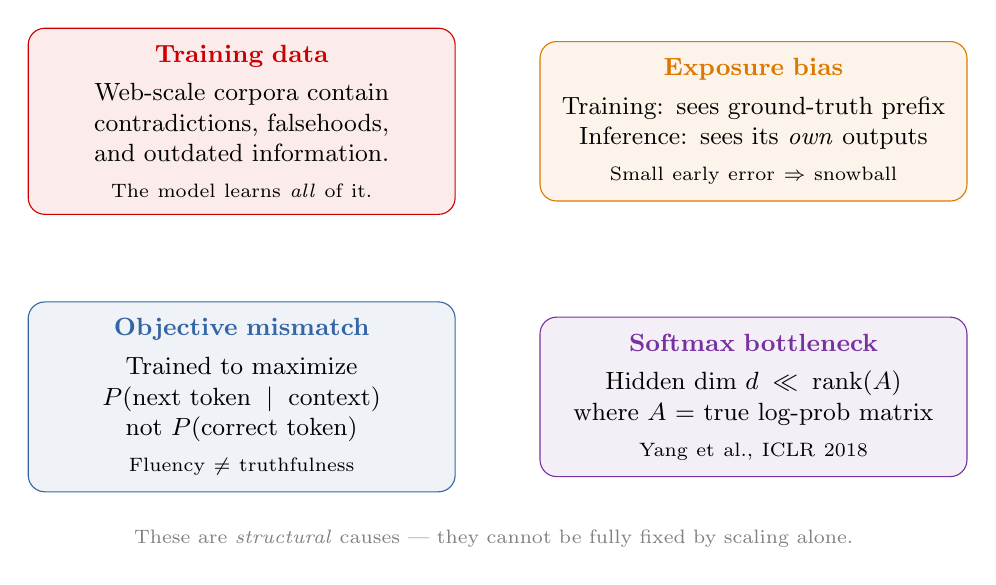
\begin{tikzpicture}
  % 4 cause boxes
  \node[draw=sampred, fill=sampred!8, rounded corners=6pt, text width=5cm, align=center, inner sep=6pt, font=\small] at (-3, 2) {
    \textbf{\textcolor{sampred}{Training data}}\\[3pt]
    Web-scale corpora contain\\contradictions, falsehoods,\\and outdated information.\\[2pt]
    {\scriptsize The model learns \emph{all} of it.}
  };
  \node[draw=orange1, fill=orange1!8, rounded corners=6pt, text width=5cm, align=center, inner sep=6pt, font=\small] at (3.5, 2) {
    \textbf{\textcolor{orange1}{Exposure bias}}\\[3pt]
    Training: sees ground-truth prefix\\Inference: sees its \emph{own} outputs\\[2pt]
    {\scriptsize Small early error $\Rightarrow$ snowball}
  };
  \node[draw=popblue, fill=popblue!8, rounded corners=6pt, text width=5cm, align=center, inner sep=6pt, font=\small] at (-3, -1.5) {
    \textbf{\textcolor{popblue}{Objective mismatch}}\\[3pt]
    Trained to maximize\\$P(\text{next token} \mid \text{context})$\\not $P(\text{correct token})$\\[2pt]
    {\scriptsize Fluency $\neq$ truthfulness}
  };
  \node[draw=violet1, fill=violet1!8, rounded corners=6pt, text width=5cm, align=center, inner sep=6pt, font=\small] at (3.5, -1.5) {
    \textbf{\textcolor{violet1}{Softmax bottleneck}}\\[3pt]
    Hidden dim $d \ll \text{rank}(A)$\\where $A$ = true log-prob matrix\\[2pt]
    {\scriptsize Yang et al., ICLR 2018}
  };

  % Connecting idea
  \node[font=\scriptsize, text=gray, text width=10cm, align=center] at (0.2, -3.3) {
    These are \emph{structural} causes --- they cannot be fully fixed by scaling alone.
  };
\end{tikzpicture}
\end{center}
\end{frame}

% ============================================================
% WHY — GENERATION DYNAMICS
% ============================================================
\begin{frame}
\frametitle{Why LLMs hallucinate --- generation dynamics}

\begin{center}
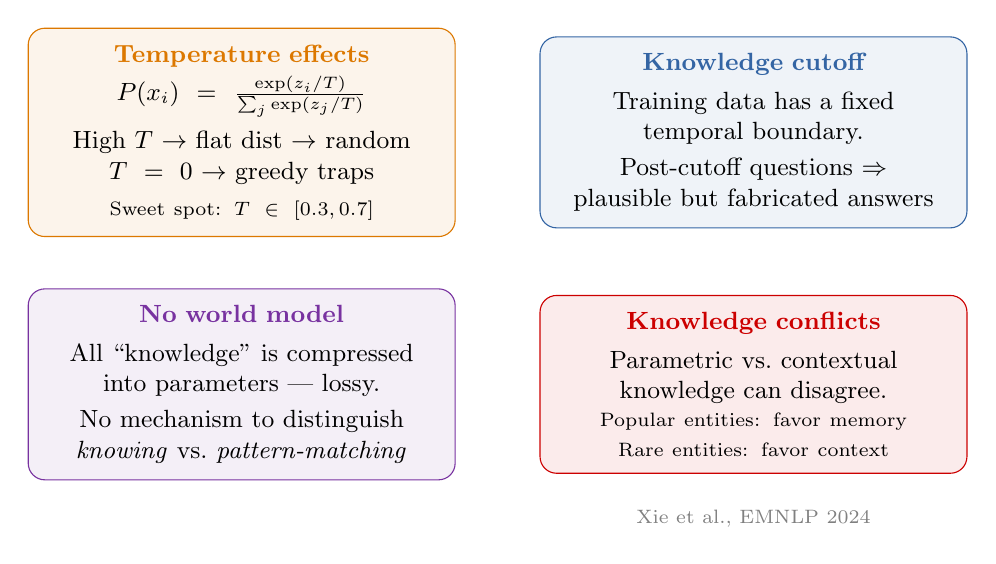
\begin{tikzpicture}
  % Temperature
  \node[draw=orange1, fill=orange1!8, rounded corners=6pt, text width=5cm, align=center, inner sep=6pt, font=\small] at (-3, 2.2) {
    \textbf{\textcolor{orange1}{Temperature effects}}\\[3pt]
    $P(x_i) = \frac{\exp(z_i / T)}{\sum_j \exp(z_j / T)}$\\[4pt]
    High $T$ $\to$ flat dist $\to$ random\\
    $T = 0$ $\to$ greedy traps\\[2pt]
    {\scriptsize Sweet spot: $T \in [0.3, 0.7]$}
  };

  % Knowledge cutoff
  \node[draw=popblue, fill=popblue!8, rounded corners=6pt, text width=5cm, align=center, inner sep=6pt, font=\small] at (3.5, 2.2) {
    \textbf{\textcolor{popblue}{Knowledge cutoff}}\\[3pt]
    Training data has a fixed\\temporal boundary.\\[2pt]
    Post-cutoff questions $\Rightarrow$\\plausible but fabricated answers
  };

  % No world model
  \node[draw=violet1, fill=violet1!8, rounded corners=6pt, text width=5cm, align=center, inner sep=6pt, font=\small] at (-3, -1) {
    \textbf{\textcolor{violet1}{No world model}}\\[3pt]
    All ``knowledge'' is compressed\\into parameters --- lossy.\\[2pt]
    No mechanism to distinguish\\\emph{knowing} vs.\ \emph{pattern-matching}
  };

  % Knowledge conflicts
  \node[draw=sampred, fill=sampred!8, rounded corners=6pt, text width=5cm, align=center, inner sep=6pt, font=\small] at (3.5, -1) {
    \textbf{\textcolor{sampred}{Knowledge conflicts}}\\[3pt]
    Parametric vs.\ contextual\\knowledge can disagree.\\[2pt]
    {\scriptsize Popular entities: favor memory\\Rare entities: favor context}
  };

  \node[font=\scriptsize, text=gray] at (3.5, -2.7) {Xie et al., EMNLP 2024};
\end{tikzpicture}
\end{center}
\end{frame}

% ============================================================
% THE CONFIDENCE PROBLEM
% ============================================================
\begin{frame}
\frametitle{The confidence problem}

\vspace{-0.3cm}
\begin{center}
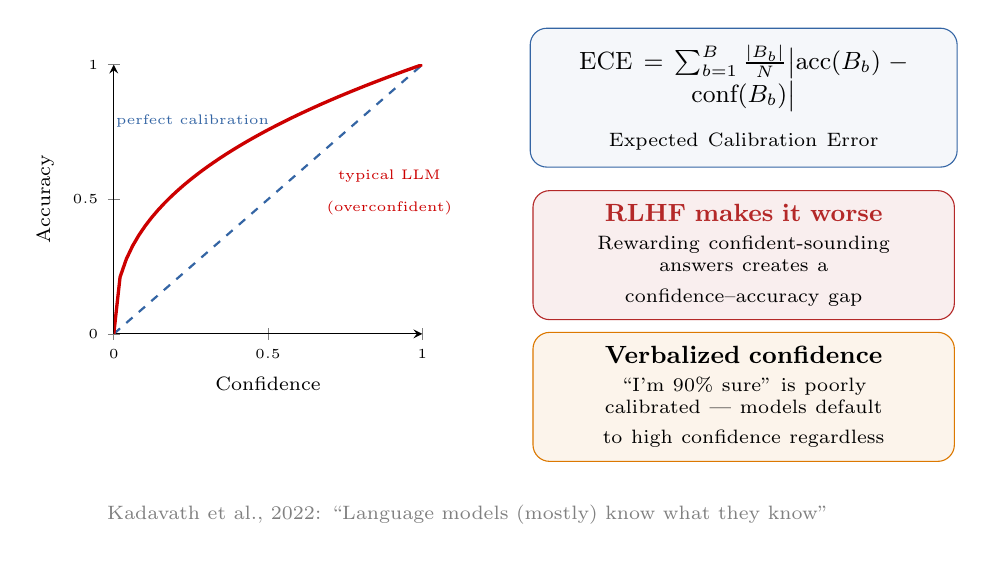
\begin{tikzpicture}
  % Calibration plot
  \begin{axis}[
    at={(-4.5cm, -0.5cm)},
    width=5.5cm, height=5cm,
    xlabel={\scriptsize Confidence},
    ylabel={\scriptsize Accuracy},
    xmin=0, xmax=1, ymin=0, ymax=1,
    xtick={0, 0.5, 1},
    ytick={0, 0.5, 1},
    axis lines=left,
    tick label style={font=\tiny},
    label style={font=\scriptsize},
  ]
    % Perfect calibration
    \addplot[popblue, thick, dashed, domain=0:1] {x};
    % Overconfident model
    \addplot[sampred, very thick, domain=0:1, samples=50] {x^0.4};
  \end{axis}

  \node[font=\tiny, text=popblue] at (-3.5, 2.2) {perfect calibration};
  \node[font=\tiny, text=sampred] at (-1, 1.5) {typical LLM};
  \node[font=\tiny, text=sampred] at (-1, 1.1) {(overconfident)};

  % ECE formula
  \node[draw=popblue, fill=popblue!5, rounded corners=6pt, inner sep=6pt, text width=5cm, align=center] at (3.5, 2.5) {
    {\small $\text{ECE} = \sum_{b=1}^{B} \frac{|B_b|}{N} \big|\text{acc}(B_b) - \text{conf}(B_b)\big|$}\\[4pt]
    {\scriptsize Expected Calibration Error}
  };

  % RLHF overconfidence
  \node[draw=warnred, fill=warnred!8, rounded corners=6pt, text width=5cm, align=center, inner sep=5pt, font=\small] at (3.5, 0.5) {
    \textbf{\textcolor{warnred}{RLHF makes it worse}}\\[2pt]
    {\scriptsize Rewarding confident-sounding\\answers creates a\\confidence--accuracy gap}
  };

  % Verbalized confidence
  \node[draw=orange1, fill=orange1!8, rounded corners=6pt, text width=5cm, align=center, inner sep=5pt, font=\small] at (3.5, -1.3) {
    \textbf{Verbalized confidence}\\[2pt]
    {\scriptsize ``I'm 90\% sure'' is poorly\\calibrated --- models default\\to high confidence regardless}
  };

  \node[font=\scriptsize, text=gray] at (0, -2.8) {Kadavath et al., 2022: ``Language models (mostly) know what they know''};
\end{tikzpicture}
\end{center}
\end{frame}

% ============================================================
% REAL-WORLD CONSEQUENCES
% ============================================================
\begin{frame}
\frametitle{Real-world consequences}

\begin{center}
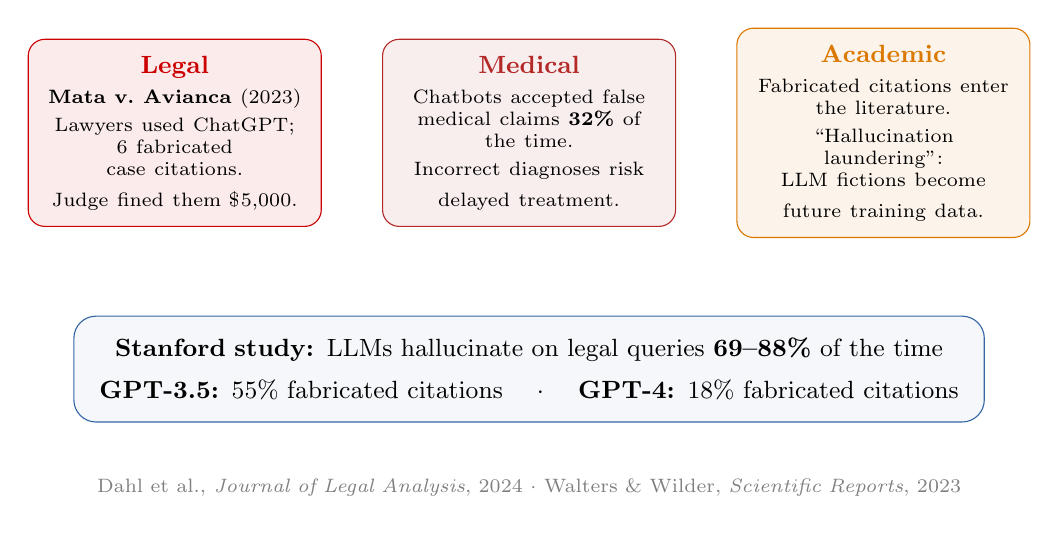
\begin{tikzpicture}
  % Legal
  \node[draw=sampred, fill=sampred!8, rounded corners=6pt, text width=3.3cm, align=center, inner sep=6pt, font=\small] at (-4.5, 1.5) {
    \textbf{\textcolor{sampred}{Legal}}\\[3pt]
    {\scriptsize \textbf{Mata v.\ Avianca} (2023)\\[2pt]
    Lawyers used ChatGPT;\\6 fabricated case citations.\\Judge fined them \$5,000.}
  };

  % Medical
  \node[draw=warnred, fill=warnred!8, rounded corners=6pt, text width=3.3cm, align=center, inner sep=6pt, font=\small] at (0, 1.5) {
    \textbf{\textcolor{warnred}{Medical}}\\[3pt]
    {\scriptsize Chatbots accepted false\\medical claims \textbf{32\%} of\\the time.\\[2pt]
    Incorrect diagnoses risk\\delayed treatment.}
  };

  % Academic
  \node[draw=orange1, fill=orange1!8, rounded corners=6pt, text width=3.3cm, align=center, inner sep=6pt, font=\small] at (4.5, 1.5) {
    \textbf{\textcolor{orange1}{Academic}}\\[3pt]
    {\scriptsize Fabricated citations enter\\the literature.\\[2pt]
    ``Hallucination laundering'':\\LLM fictions become\\future training data.}
  };

  % Stats
  \node[draw=popblue, fill=popblue!5, rounded corners=8pt, text width=11cm, align=center, inner sep=8pt, font=\small] at (0, -1.5) {
    \textbf{Stanford study:} LLMs hallucinate on legal queries \textbf{69--88\%} of the time\\[4pt]
    \textbf{GPT-3.5:} 55\% fabricated citations \quad $\cdot$ \quad
    \textbf{GPT-4:} 18\% fabricated citations
  };

  % Bottom
  \node[font=\scriptsize, text=gray, text width=11cm, align=center] at (0, -3) {
    Dahl et al., \emph{Journal of Legal Analysis}, 2024 $\cdot$ Walters \& Wilder, \emph{Scientific Reports}, 2023
  };
\end{tikzpicture}
\end{center}
\end{frame}

% ============================================================
% DETECTION: SELFCHECKGPT
% ============================================================
\begin{frame}
\frametitle{Detection: SelfCheckGPT}

\vspace{-0.1cm}
\begin{center}
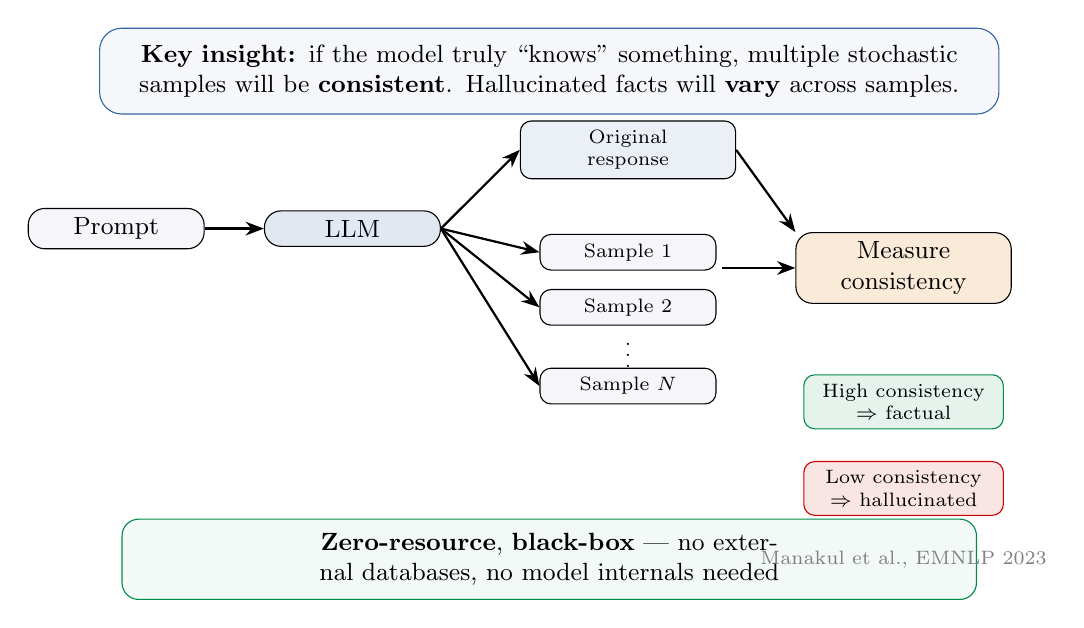
\begin{tikzpicture}
  % Key insight
  \node[draw=popblue, fill=popblue!5, rounded corners=8pt, text width=11cm, align=center, inner sep=6pt, font=\small] at (0, 3) {
    \textbf{Key insight:} if the model truly ``knows'' something, multiple stochastic samples will be \textbf{consistent}. Hallucinated facts will \textbf{vary} across samples.
  };

  % Pipeline
  \node[draw, rounded corners=6pt, fill=lightbg, font=\small, text width=2cm, align=center] (prompt) at (-5.5, 1) {Prompt};
  \node[draw, rounded corners=6pt, fill=popblue!15, font=\small, text width=2cm, align=center] (model) at (-2.5, 1) {LLM};
  \draw[-Stealth, thick] (prompt) -- (model);

  % Original response
  \node[draw, rounded corners=4pt, fill=popblue!10, font=\scriptsize, text width=2.5cm, align=center] (orig) at (1, 2) {Original\\response};
  \draw[-Stealth, thick] (model.east) -- (orig.west);

  % Stochastic samples
  \node[draw, rounded corners=4pt, fill=lightbg, font=\scriptsize, text width=2cm, align=center] (s1) at (1, 0.7) {Sample 1};
  \node[draw, rounded corners=4pt, fill=lightbg, font=\scriptsize, text width=2cm, align=center] (s2) at (1, 0) {Sample 2};
  \node[font=\scriptsize] at (1, -0.5) {$\vdots$};
  \node[draw, rounded corners=4pt, fill=lightbg, font=\scriptsize, text width=2cm, align=center] (sn) at (1, -1) {Sample $N$};

  \draw[-Stealth, thick] (model.east) -- (s1.west);
  \draw[-Stealth, thick] (model.east) -- (s2.west);
  \draw[-Stealth, thick] (model.east) -- (sn.west);

  % Compare
  \node[draw, rounded corners=6pt, fill=orange1!15, font=\small, text width=2.5cm, align=center] (comp) at (4.5, 0.5) {Measure\\consistency};
  \draw[-Stealth, thick] (orig.east) -- (comp.north west);
  \draw[-Stealth, thick] (2.2, 0.5) -- (comp.west);

  % Result
  \node[draw=paramgreen, fill=paramgreen!10, rounded corners=4pt, font=\scriptsize, text width=2.3cm, align=center] at (4.5, -1.2) {High consistency\\$\Rightarrow$ factual};
  \node[draw=sampred, fill=sampred!10, rounded corners=4pt, font=\scriptsize, text width=2.3cm, align=center] at (4.5, -2.3) {Low consistency\\$\Rightarrow$ hallucinated};

  % Properties
  \node[draw=paramgreen, fill=paramgreen!5, rounded corners=6pt, text width=10.5cm, align=center, inner sep=5pt, font=\small] at (0, -3.2) {
    \textbf{Zero-resource}, \textbf{black-box} --- no external databases, no model internals needed
  };

  \node[font=\scriptsize, text=gray] at (4.5, -3.2) {Manakul et al., EMNLP 2023};
\end{tikzpicture}
\end{center}
\end{frame}

% ============================================================
% DETECTION: SEMANTIC ENTROPY
% ============================================================
\begin{frame}
\frametitle{Detection: Semantic Entropy}

\vspace{-0.2cm}
\begin{center}
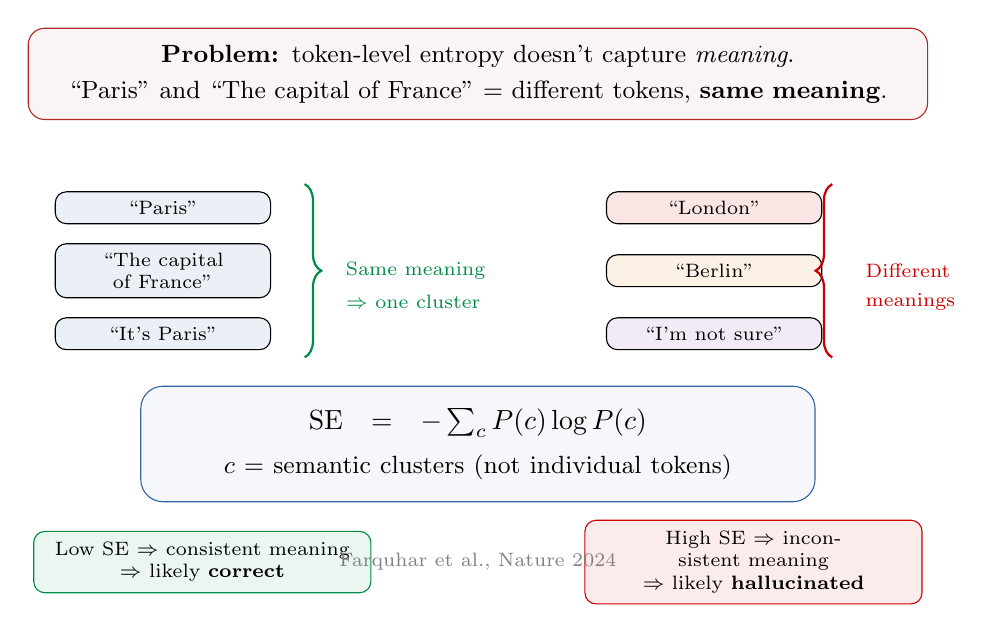
\begin{tikzpicture}
  % Problem with token entropy
  \node[draw=warnred, fill=warnred!5, rounded corners=6pt, text width=11cm, align=center, inner sep=6pt, font=\small] at (0, 3) {
    \textbf{Problem:} token-level entropy doesn't capture \emph{meaning}.\\[2pt]
    ``Paris'' and ``The capital of France'' = different tokens, \textbf{same meaning}.
  };

  % Visual: tokens vs meanings
  \node[draw, rounded corners=4pt, fill=popblue!10, font=\scriptsize, text width=2.5cm, align=center] at (-4, 1.3) {``Paris''};
  \node[draw, rounded corners=4pt, fill=popblue!10, font=\scriptsize, text width=2.5cm, align=center] at (-4, 0.5) {``The capital\\of France''};
  \node[draw, rounded corners=4pt, fill=popblue!10, font=\scriptsize, text width=2.5cm, align=center] at (-4, -0.3) {``It's Paris''};

  \draw[decorate, decoration={brace, mirror, amplitude=6pt}, thick, paramgreen] (-2.2, -0.6) -- (-2.2, 1.6);
  \node[font=\scriptsize, text=paramgreen, anchor=west] at (-1.8, 0.5) {Same meaning};
  \node[font=\scriptsize, text=paramgreen, anchor=west] at (-1.8, 0.1) {$\Rightarrow$ one cluster};

  % Different meaning
  \node[draw, rounded corners=4pt, fill=sampred!10, font=\scriptsize, text width=2.5cm, align=center] at (3, 1.3) {``London''};
  \node[draw, rounded corners=4pt, fill=orange1!10, font=\scriptsize, text width=2.5cm, align=center] at (3, 0.5) {``Berlin''};
  \node[draw, rounded corners=4pt, fill=violet1!10, font=\scriptsize, text width=2.5cm, align=center] at (3, -0.3) {``I'm not sure''};

  \draw[decorate, decoration={brace, amplitude=6pt}, thick, sampred] (4.5, -0.6) -- (4.5, 1.6);
  \node[font=\scriptsize, text=sampred, anchor=west] at (4.8, 0.5) {Different};
  \node[font=\scriptsize, text=sampred, anchor=west] at (4.8, 0.1) {meanings};

  % Formula
  \node[draw=popblue, fill=popblue!5, rounded corners=8pt, inner sep=8pt, text width=8cm, align=center] at (0, -1.7) {
    {\normalsize $\text{SE} = -\sum_{c} P(c) \log P(c)$}\\[4pt]
    {\small $c$ = semantic clusters (not individual tokens)}
  };

  % Interpretation
  \node[draw=paramgreen, fill=paramgreen!8, rounded corners=4pt, text width=4cm, align=center, inner sep=4pt, font=\scriptsize] at (-3.5, -3.2) {
    Low SE $\Rightarrow$ consistent meaning\\$\Rightarrow$ likely \textbf{correct}
  };
  \node[draw=sampred, fill=sampred!8, rounded corners=4pt, text width=4cm, align=center, inner sep=4pt, font=\scriptsize] at (3.5, -3.2) {
    High SE $\Rightarrow$ inconsistent meaning\\$\Rightarrow$ likely \textbf{hallucinated}
  };

  \node[font=\scriptsize, text=gray] at (0, -3.2) {Farquhar et al., Nature 2024};
\end{tikzpicture}
\end{center}
\end{frame}

% ============================================================
% DETECTION: DoLa & COMPARISON
% ============================================================
\begin{frame}
\frametitle{Detection methods compared}

\vspace{-0.5cm}
\begin{center}
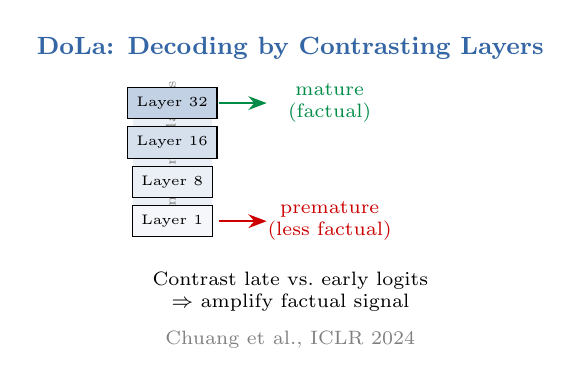
\begin{tikzpicture}
  % DoLa diagram
  \node[font=\small\bfseries, text=popblue] at (-3.5, 2.8) {DoLa: Decoding by Contrasting Layers};

  % Layer stack
  \fill[popblue!10] (-5.5, 0.5) rectangle (-4.5, 2.3);
  \node[font=\tiny, text=gray, rotate=90] at (-5, 1.4) {Transformer layers};

  \node[draw, fill=popblue!30, minimum width=0.8cm, minimum height=0.4cm, font=\tiny] at (-5, 2.1) {Layer 32};
  \node[draw, fill=popblue!20, minimum width=0.8cm, minimum height=0.4cm, font=\tiny] at (-5, 1.6) {Layer 16};
  \node[draw, fill=popblue!10, minimum width=0.8cm, minimum height=0.4cm, font=\tiny] at (-5, 1.1) {Layer 8};
  \node[draw, fill=popblue!5, minimum width=0.8cm, minimum height=0.4cm, font=\tiny] at (-5, 0.6) {Layer 1};

  \node[font=\scriptsize, text=paramgreen, text width=2.5cm, align=center] at (-3, 2.1) {mature\\(factual)};
  \node[font=\scriptsize, text=sampred, text width=2.5cm, align=center] at (-3, 0.6) {premature\\(less factual)};

  \draw[-Stealth, thick, paramgreen] (-4.4, 2.1) -- (-3.8, 2.1);
  \draw[-Stealth, thick, sampred] (-4.4, 0.6) -- (-3.8, 0.6);

  \node[font=\scriptsize, text width=3.5cm, align=center] at (-3.5, -0.3) {Contrast late vs.\ early logits\\$\Rightarrow$ amplify factual signal};
  \node[font=\scriptsize, text=gray] at (-3.5, -0.9) {Chuang et al., ICLR 2024};
\end{tikzpicture}

\vspace{0.1cm}
\renewcommand{\arraystretch}{1.3}
{\small
\begin{tabular}{>{\bfseries}l c l}
  \textbf{Method} & \textbf{Access} & \textbf{Key idea} \\
  \hline
  \textcolor{popblue}{SelfCheckGPT} & Black-box & Multi-sample consistency \\[1pt]
  \textcolor{paramgreen}{Semantic Entropy} & Black-box & Meaning-level uncertainty \\[1pt]
  \textcolor{orange1}{DoLa} & White-box & Layer-contrastive decoding \\[1pt]
  \textcolor{violet1}{Logit-based} & White-box & Token probability thresholds \\[1pt]
  \textcolor{sampred}{NLI-based} & Black-box & Entailment checking vs.\ source \\
  \hline
\end{tabular}
}
\end{center}
\end{frame}

% ============================================================
% MITIGATION: RAG
% ============================================================
\begin{frame}
\frametitle{Mitigation: RAG as grounding}

\begin{center}
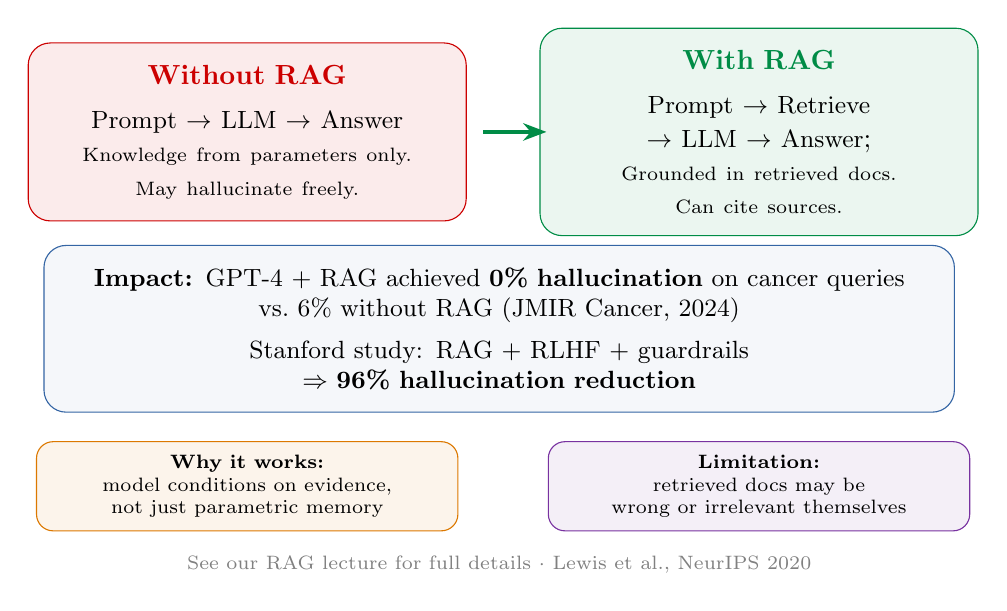
\begin{tikzpicture}
  % Without RAG
  \node[draw=sampred, fill=sampred!8, rounded corners=8pt, text width=5cm, align=center, inner sep=8pt] at (-3, 2) {
    \textbf{\textcolor{sampred}{Without RAG}}\\[4pt]
    {\small Prompt $\to$ LLM $\to$ Answer}\\[4pt]
    {\scriptsize Knowledge from parameters only.\\May hallucinate freely.}
  };

  % With RAG
  \node[draw=paramgreen, fill=paramgreen!8, rounded corners=8pt, text width=5cm, align=center, inner sep=8pt] at (3.5, 2) {
    \textbf{\textcolor{paramgreen}{With RAG}}\\[4pt]
    {\small Prompt $\to$ Retrieve $\to$ LLM $\to$ Answer};\\[4pt]
    {\scriptsize Grounded in retrieved docs.\\Can cite sources.}
  };

  \draw[-Stealth, very thick, paramgreen] (0, 2) -- (0.8, 2);

  % Impact
  \node[draw=popblue, fill=popblue!5, rounded corners=8pt, text width=11cm, align=center, inner sep=8pt, font=\small] at (0.2, -0.5) {
    \textbf{Impact:} GPT-4 + RAG achieved \textbf{0\% hallucination} on cancer queries\\
    vs.\ 6\% without RAG (JMIR Cancer, 2024)\\[4pt]
    Stanford study: RAG + RLHF + guardrails $\Rightarrow$ \textbf{96\% hallucination reduction}
  };

  % How it helps
  \node[draw=orange1, fill=orange1!8, rounded corners=6pt, text width=5cm, align=center, inner sep=5pt, font=\scriptsize] at (-3, -2.5) {
    \textbf{Why it works:}\\model conditions on evidence,\\not just parametric memory
  };
  \node[draw=violet1, fill=violet1!8, rounded corners=6pt, text width=5cm, align=center, inner sep=5pt, font=\scriptsize] at (3.5, -2.5) {
    \textbf{Limitation:}\\retrieved docs may be\\wrong or irrelevant themselves
  };

  \node[font=\scriptsize, text=gray] at (0.2, -3.5) {See our RAG lecture for full details $\cdot$ Lewis et al., NeurIPS 2020};
\end{tikzpicture}
\end{center}
\end{frame}

% ============================================================
% MITIGATION: CHAIN-OF-VERIFICATION
% ============================================================
\begin{frame}
\frametitle{Mitigation: Chain-of-Verification (CoVe)}

\begin{center}
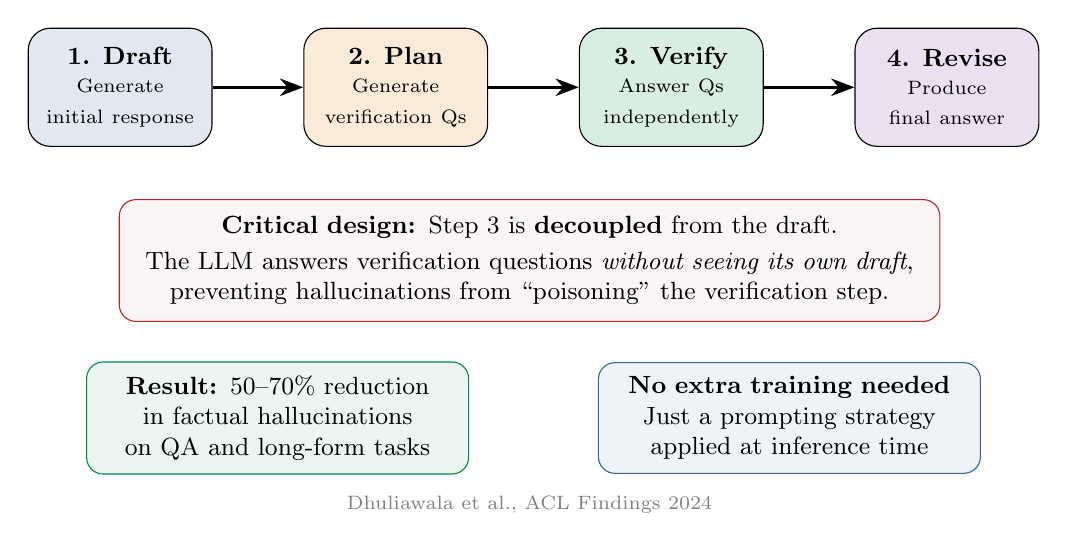
\begin{tikzpicture}
  % 4-step pipeline
  \node[draw, rounded corners=8pt, fill=popblue!15, minimum width=2.3cm, minimum height=1.5cm, font=\small, text width=2.1cm, align=center] (s1) at (-5, 2) {
    \textbf{1. Draft}\\[2pt]
    {\scriptsize Generate\\initial response}
  };
  \node[draw, rounded corners=8pt, fill=orange1!15, minimum width=2.3cm, minimum height=1.5cm, font=\small, text width=2.1cm, align=center] (s2) at (-1.5, 2) {
    \textbf{2. Plan}\\[2pt]
    {\scriptsize Generate\\verification Qs}
  };
  \node[draw, rounded corners=8pt, fill=paramgreen!15, minimum width=2.3cm, minimum height=1.5cm, font=\small, text width=2.1cm, align=center] (s3) at (2, 2) {
    \textbf{3. Verify}\\[2pt]
    {\scriptsize Answer Qs\\independently}
  };
  \node[draw, rounded corners=8pt, fill=violet1!15, minimum width=2.3cm, minimum height=1.5cm, font=\small, text width=2.1cm, align=center] (s4) at (5.5, 2) {
    \textbf{4. Revise}\\[2pt]
    {\scriptsize Produce\\final answer}
  };

  \draw[-Stealth, very thick] (s1) -- (s2);
  \draw[-Stealth, very thick] (s2) -- (s3);
  \draw[-Stealth, very thick] (s3) -- (s4);

  % The key design choice
  \node[draw=warnred, fill=warnred!5, rounded corners=6pt, text width=10cm, align=center, inner sep=6pt, font=\small] at (0.2, -0.2) {
    \textbf{Critical design:} Step 3 is \textbf{decoupled} from the draft.\\[2pt]
    The LLM answers verification questions \emph{without seeing its own draft},\\
    preventing hallucinations from ``poisoning'' the verification step.
  };

  % Results
  \node[draw=paramgreen, fill=paramgreen!8, rounded corners=6pt, text width=4.5cm, align=center, inner sep=5pt, font=\small] at (-3, -2.2) {
    \textbf{Result:} 50--70\% reduction\\in factual hallucinations\\on QA and long-form tasks
  };
  \node[draw=popblue, fill=popblue!8, rounded corners=6pt, text width=4.5cm, align=center, inner sep=5pt, font=\small] at (3.5, -2.2) {
    \textbf{No extra training needed}\\Just a prompting strategy\\applied at inference time
  };

  \node[font=\scriptsize, text=gray] at (0.2, -3.3) {Dhuliawala et al., ACL Findings 2024};
\end{tikzpicture}
\end{center}
\end{frame}

% ============================================================
% MITIGATION: SELF-CONSISTENCY
% ============================================================
\begin{frame}
\frametitle{Mitigation: Self-Consistency \& constrained decoding}

\begin{center}
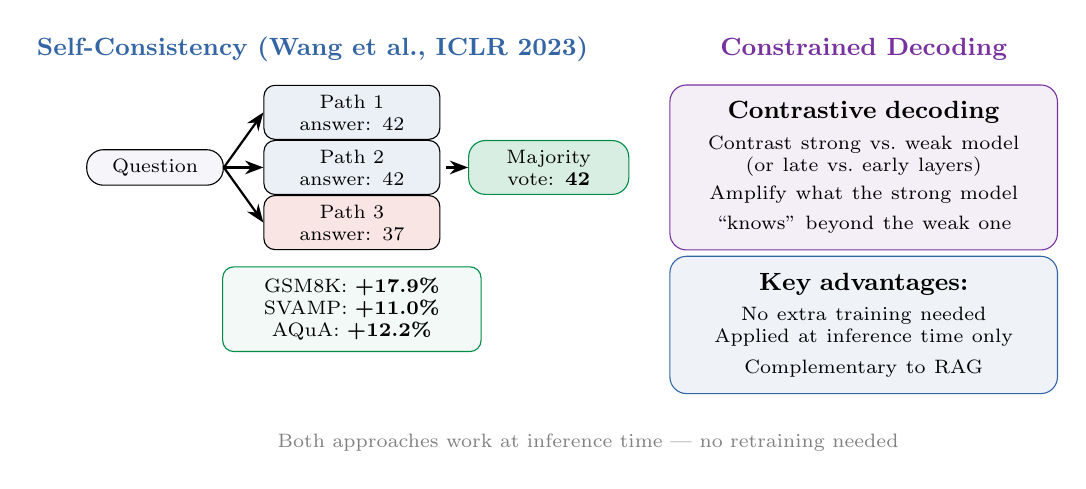
\begin{tikzpicture}
  % Self-consistency diagram
  \node[font=\small\bfseries, text=popblue] at (-3.5, 3) {Self-Consistency (Wang et al., ICLR 2023)};

  \node[draw, rounded corners=6pt, fill=lightbg, font=\scriptsize, text width=1.5cm, align=center] (q) at (-5.5, 1.5) {Question};

  % Multiple paths
  \node[draw, rounded corners=4pt, fill=popblue!10, font=\scriptsize, text width=2cm, align=center] (p1) at (-3, 2.2) {Path 1\\answer: 42};
  \node[draw, rounded corners=4pt, fill=popblue!10, font=\scriptsize, text width=2cm, align=center] (p2) at (-3, 1.5) {Path 2\\answer: 42};
  \node[draw, rounded corners=4pt, fill=sampred!10, font=\scriptsize, text width=2cm, align=center] (p3) at (-3, 0.8) {Path 3\\answer: 37};

  \draw[-Stealth, thick] (q.east) -- (p1.west);
  \draw[-Stealth, thick] (q.east) -- (p2.west);
  \draw[-Stealth, thick] (q.east) -- (p3.west);

  % Majority vote
  \node[draw=paramgreen, fill=paramgreen!15, rounded corners=6pt, font=\scriptsize, text width=1.8cm, align=center] (vote) at (-0.5, 1.5) {Majority\\vote: \textbf{42}};
  \draw[-Stealth, thick] (-1.8, 1.5) -- (vote.west);

  % Results
  \node[draw=paramgreen, fill=paramgreen!5, rounded corners=4pt, text width=3cm, align=center, inner sep=4pt, font=\scriptsize] at (-3, -0.3) {
    GSM8K: \textbf{+17.9\%}\\SVAMP: \textbf{+11.0\%}\\AQuA: \textbf{+12.2\%}
  };

  % Constrained decoding
  \node[font=\small\bfseries, text=violet1] at (3.5, 3) {Constrained Decoding};

  \node[draw=violet1, fill=violet1!8, rounded corners=6pt, text width=4.5cm, align=center, inner sep=6pt, font=\small] at (3.5, 1.5) {
    \textbf{Contrastive decoding}\\[3pt]
    {\scriptsize Contrast strong vs.\ weak model\\(or late vs.\ early layers)\\[2pt]
    Amplify what the strong model\\``knows'' beyond the weak one}
  };

  \node[draw=popblue, fill=popblue!8, rounded corners=6pt, text width=4.5cm, align=center, inner sep=6pt, font=\small] at (3.5, -0.5) {
    \textbf{Key advantages:}\\[3pt]
    {\scriptsize No extra training needed\\Applied at inference time only\\Complementary to RAG}
  };

  \node[font=\scriptsize, text=gray, text width=10cm, align=center] at (0, -2) {
    Both approaches work at inference time --- no retraining needed
  };
\end{tikzpicture}
\end{center}
\end{frame}

% ============================================================
% GROUNDING & ATTRIBUTION
% ============================================================
\begin{frame}
\frametitle{Grounding \& attribution}

\begin{center}
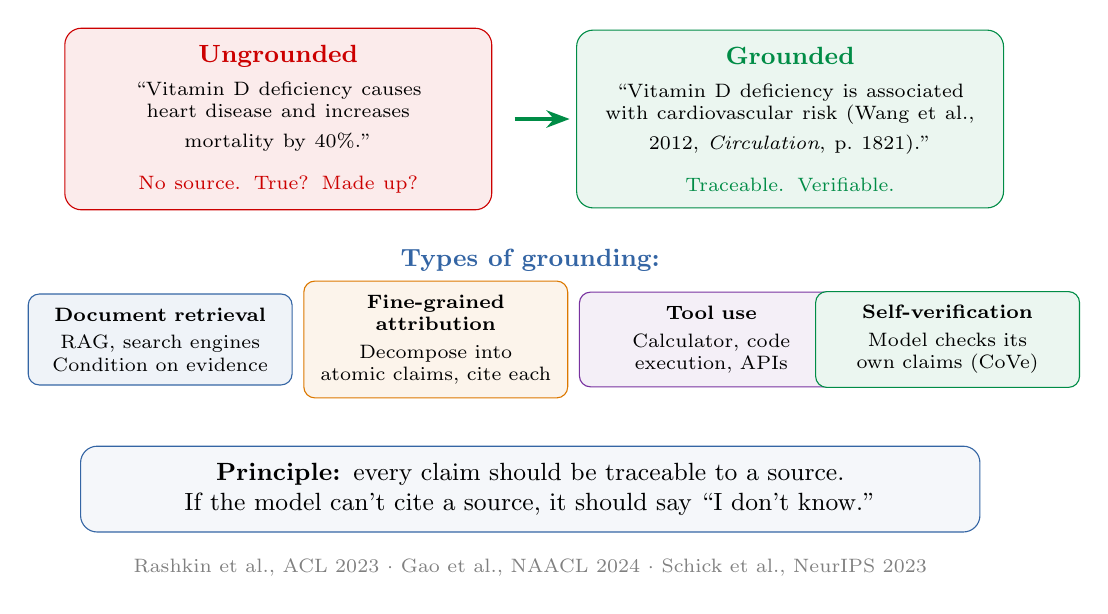
\begin{tikzpicture}
  % Ungrounded vs grounded
  \node[draw=sampred, fill=sampred!8, rounded corners=6pt, text width=5cm, align=center, inner sep=6pt, font=\small] at (-3, 2.5) {
    \textbf{\textcolor{sampred}{Ungrounded}}\\[4pt]
    {\scriptsize ``Vitamin D deficiency causes\\heart disease and increases\\mortality by 40\%.''}\\[4pt]
    {\scriptsize \textcolor{sampred}{No source. True? Made up?}}
  };
  \node[draw=paramgreen, fill=paramgreen!8, rounded corners=6pt, text width=5cm, align=center, inner sep=6pt, font=\small] at (3.5, 2.5) {
    \textbf{\textcolor{paramgreen}{Grounded}}\\[4pt]
    {\scriptsize ``Vitamin D deficiency is associated\\with cardiovascular risk (Wang et al.,\\2012, \emph{Circulation}, p.\ 1821).''}\\[4pt]
    {\scriptsize \textcolor{paramgreen}{Traceable. Verifiable.}}
  };

  \draw[-Stealth, very thick, paramgreen] (0, 2.5) -- (0.7, 2.5);

  % Attribution types
  \node[font=\small\bfseries, text=popblue] at (0.2, 0.7) {Types of grounding:};

  \node[draw=popblue, fill=popblue!8, rounded corners=4pt, text width=3cm, align=center, inner sep=5pt, font=\scriptsize] at (-4.5, -0.3) {
    \textbf{Document retrieval}\\[2pt]
    RAG, search engines\\Condition on evidence
  };
  \node[draw=orange1, fill=orange1!8, rounded corners=4pt, text width=3cm, align=center, inner sep=5pt, font=\scriptsize] at (-1, -0.3) {
    \textbf{Fine-grained\\attribution}\\[2pt]
    Decompose into\\atomic claims, cite each
  };
  \node[draw=violet1, fill=violet1!8, rounded corners=4pt, text width=3cm, align=center, inner sep=5pt, font=\scriptsize] at (2.5, -0.3) {
    \textbf{Tool use}\\[2pt]
    Calculator, code\\execution, APIs
  };
  \node[draw=paramgreen, fill=paramgreen!8, rounded corners=4pt, text width=3cm, align=center, inner sep=5pt, font=\scriptsize] at (5.5, -0.3) {
    \textbf{Self-verification}\\[2pt]
    Model checks its\\own claims (CoVe)
  };

  % Key principle
  \node[draw=popblue, fill=popblue!5, rounded corners=6pt, text width=11cm, align=center, inner sep=6pt, font=\small] at (0.2, -2.2) {
    \textbf{Principle:} every claim should be traceable to a source.\\If the model can't cite a source, it should say ``I don't know.''
  };

  \node[font=\scriptsize, text=gray] at (0.2, -3.2) {Rashkin et al., ACL 2023 $\cdot$ Gao et al., NAACL 2024 $\cdot$ Schick et al., NeurIPS 2023};
\end{tikzpicture}
\end{center}
\end{frame}

% ============================================================
% FAITHFULNESS VS FACTUALITY
% ============================================================
\begin{frame}
\frametitle{Faithfulness vs.\ factuality}

\begin{center}
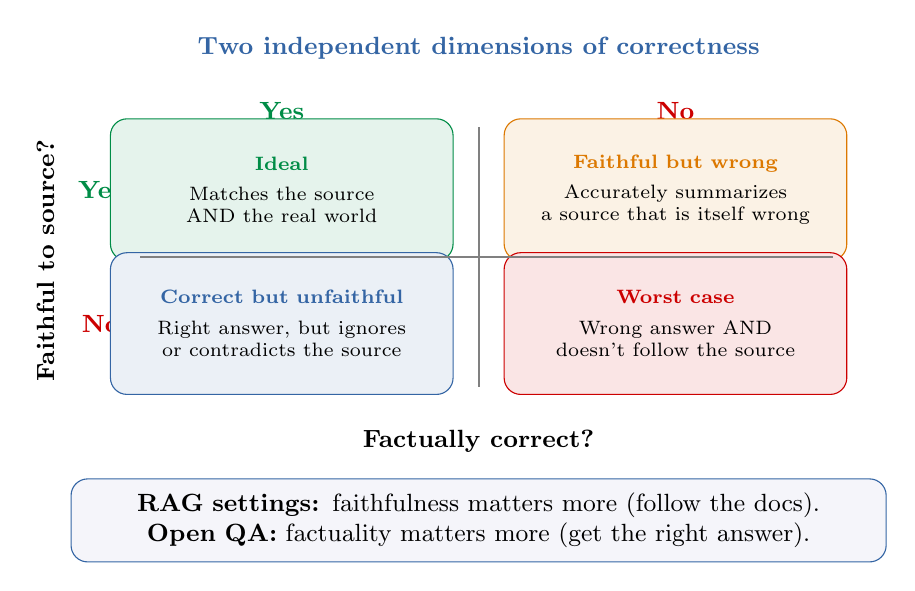
\begin{tikzpicture}
  % 2x2 grid
  % Headers
  \node[font=\small\bfseries, text=popblue] at (0, 3.5) {Two independent dimensions of correctness};

  % Axis labels
  \node[font=\small\bfseries, rotate=90] at (-5.5, 0.8) {Faithful to source?};
  \node[font=\small\bfseries] at (0, -1.5) {Factually correct?};

  % Column headers
  \node[font=\small\bfseries, text=paramgreen] at (-2.5, 2.7) {Yes};
  \node[font=\small\bfseries, text=sampred] at (2.5, 2.7) {No};

  % Row headers
  \node[font=\small\bfseries, text=paramgreen] at (-4.8, 1.7) {Yes};
  \node[font=\small\bfseries, text=sampred] at (-4.8, 0) {No};

  % Cell 1: Faithful + Factual
  \node[draw=paramgreen, fill=paramgreen!10, rounded corners=6pt, text width=4cm, minimum height=1.8cm, align=center, inner sep=5pt, font=\scriptsize] at (-2.5, 1.7) {
    \textbf{\textcolor{paramgreen}{Ideal}}\\[3pt]
    Matches the source\\AND the real world
  };

  % Cell 2: Faithful + Not factual
  \node[draw=orange1, fill=orange1!10, rounded corners=6pt, text width=4cm, minimum height=1.8cm, align=center, inner sep=5pt, font=\scriptsize] at (2.5, 1.7) {
    \textbf{\textcolor{orange1}{Faithful but wrong}}\\[3pt]
    Accurately summarizes\\a source that is itself wrong
  };

  % Cell 3: Not faithful + Factual
  \node[draw=popblue, fill=popblue!10, rounded corners=6pt, text width=4cm, minimum height=1.8cm, align=center, inner sep=5pt, font=\scriptsize] at (-2.5, 0) {
    \textbf{\textcolor{popblue}{Correct but unfaithful}}\\[3pt]
    Right answer, but ignores\\or contradicts the source
  };

  % Cell 4: Not faithful + Not factual
  \node[draw=sampred, fill=sampred!10, rounded corners=6pt, text width=4cm, minimum height=1.8cm, align=center, inner sep=5pt, font=\scriptsize] at (2.5, 0) {
    \textbf{\textcolor{sampred}{Worst case}}\\[3pt]
    Wrong answer AND\\doesn't follow the source
  };

  % Dividers
  \draw[gray, thick] (0, -0.8) -- (0, 2.5);
  \draw[gray, thick] (-4.3, 0.85) -- (4.5, 0.85);

  % Key insight
  \node[draw=popblue, fill=lightbg, rounded corners=6pt, text width=10cm, align=center, inner sep=5pt, font=\small] at (0, -2.5) {
    \textbf{RAG settings:} faithfulness matters more (follow the docs).\\
    \textbf{Open QA:} factuality matters more (get the right answer).
  };
\end{tikzpicture}
\end{center}
\end{frame}

% ============================================================
% BENCHMARKS
% ============================================================
\begin{frame}
\frametitle{Benchmarks for hallucination}

\vspace{-0.3cm}
\renewcommand{\arraystretch}{1.4}
\begin{center}
{\small
\begin{tabular}{>{\bfseries}l l c l}
  \textbf{Benchmark} & \textbf{Measures} & \textbf{Size} & \textbf{Key feature} \\
  \hline
  \textcolor{popblue}{TruthfulQA} & Imitative falsehoods & 817 Q & Inverse scaling \\[2pt]
  \textcolor{paramgreen}{FActScore} & Atomic factual precision & Per-gen & 58\% for ChatGPT (bios) \\[2pt]
  \textcolor{orange1}{HaluEval} & Hallucination detection & 35K & QA, dialogue, summary \\[2pt]
  \textcolor{violet1}{SimpleQA} & Factual QA accuracy & -- & Straightforward questions \\
  \hline
\end{tabular}
}
\end{center}

\vspace{0.2cm}
\begin{center}
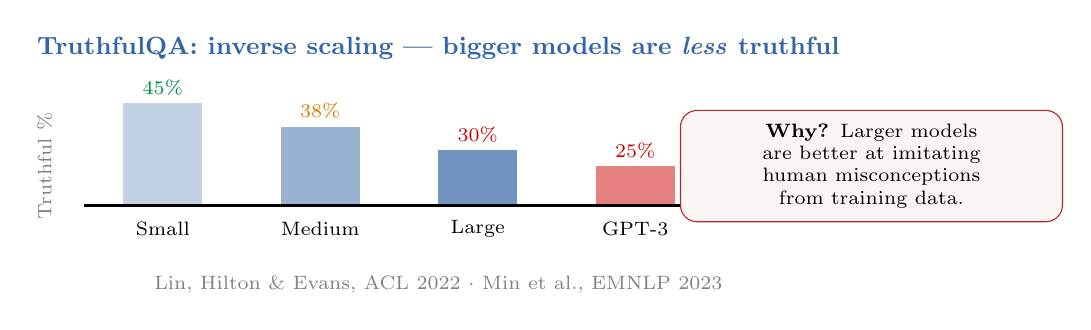
\begin{tikzpicture}
  % TruthfulQA inverse scaling
  \node[font=\small\bfseries, text=popblue] at (0, 1.5) {TruthfulQA: inverse scaling --- bigger models are \emph{less} truthful};

  % Bar chart
  \fill[popblue!30] (-4, -0.5) rectangle (-3, 0.8);
  \node[font=\scriptsize] at (-3.5, -0.8) {Small};
  \node[font=\scriptsize, text=paramgreen] at (-3.5, 1.0) {45\%};

  \fill[popblue!50] (-2, -0.5) rectangle (-1, 0.5);
  \node[font=\scriptsize] at (-1.5, -0.8) {Medium};
  \node[font=\scriptsize, text=orange1] at (-1.5, 0.7) {38\%};

  \fill[popblue!70] (0, -0.5) rectangle (1, 0.2);
  \node[font=\scriptsize] at (0.5, -0.8) {Large};
  \node[font=\scriptsize, text=sampred] at (0.5, 0.4) {30\%};

  \fill[sampred!50] (2, -0.5) rectangle (3, 0.0);
  \node[font=\scriptsize] at (2.5, -0.8) {GPT-3};
  \node[font=\scriptsize, text=sampred] at (2.5, 0.2) {25\%};

  \draw[thick] (-4.5, -0.5) -- (3.5, -0.5);
  \node[font=\scriptsize, text=gray, rotate=90] at (-5, 0) {Truthful \%};

  % Why
  \node[draw=warnred, fill=warnred!5, rounded corners=6pt, text width=4.5cm, align=center, inner sep=5pt, font=\scriptsize] at (5.5, 0) {
    \textbf{Why?} Larger models\\are better at imitating\\human misconceptions\\from training data.
  };

  \node[font=\scriptsize, text=gray] at (0, -1.5) {Lin, Hilton \& Evans, ACL 2022 $\cdot$ Min et al., EMNLP 2023};
\end{tikzpicture}
\end{center}
\end{frame}

% ============================================================
% THE FUNDAMENTAL TENSION
% ============================================================
\begin{frame}
\frametitle{The fundamental tension}

\begin{center}
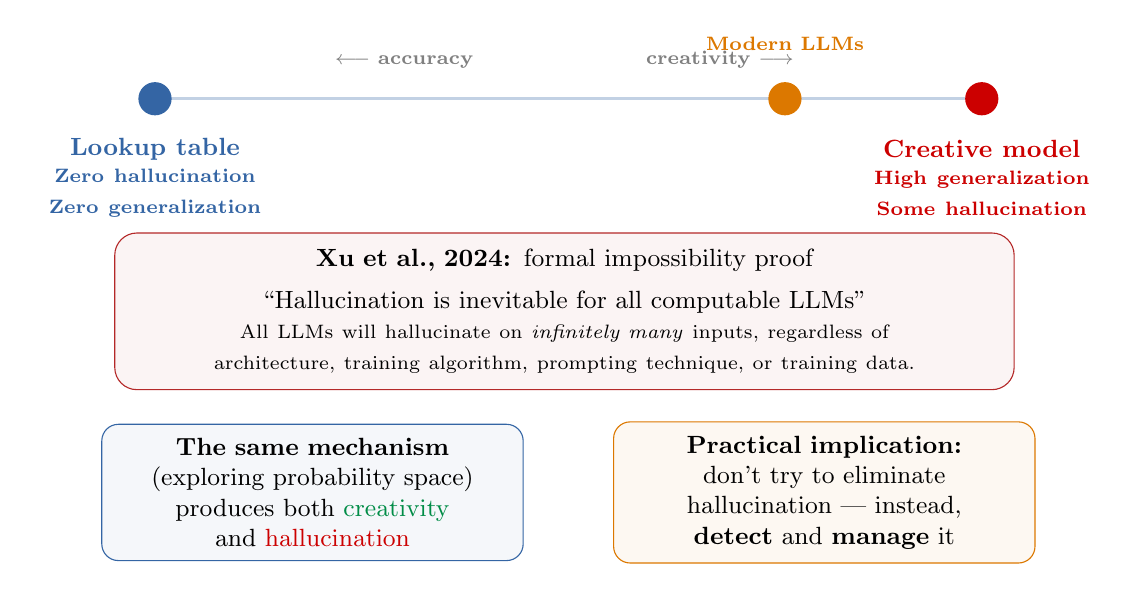
\begin{tikzpicture}
  % Spectrum
  \draw[very thick, popblue!30] (-5, 2.5) -- (5.5, 2.5);
  \fill[popblue] (-5, 2.5) circle (6pt);
  \fill[sampred] (5.5, 2.5) circle (6pt);

  % Labels
  \node[font=\small\bfseries, text=popblue, text width=3cm, align=center] at (-5, 1.5) {Lookup table\\[2pt]{\scriptsize Zero hallucination\\Zero generalization}};
  \node[font=\small\bfseries, text=sampred, text width=3cm, align=center] at (5.5, 1.5) {Creative model\\[2pt]{\scriptsize High generalization\\Some hallucination}};

  % Arrow showing the trade-off
  \node[font=\scriptsize, text=gray] at (0.2, 3.0) {$\longleftarrow$ \textbf{accuracy} \hspace{2cm} \textbf{creativity} $\longrightarrow$};

  % Where LLMs sit
  \fill[orange1] (3, 2.5) circle (6pt);
  \node[font=\scriptsize\bfseries, text=orange1] at (3, 3.2) {Modern LLMs};

  % Impossibility result
  \node[draw=warnred, fill=warnred!5, rounded corners=8pt, text width=11cm, align=center, inner sep=6pt, font=\small] at (0.2, -0.2) {
    \textbf{Xu et al., 2024:} formal impossibility proof\\[4pt]
    ``Hallucination is inevitable for all computable LLMs''\\[3pt]
    {\scriptsize All LLMs will hallucinate on \emph{infinitely many} inputs, regardless of\\architecture, training algorithm, prompting technique, or training data.}
  };

  % Why
  \node[draw=popblue, fill=popblue!5, rounded corners=6pt, text width=5cm, align=center, inner sep=5pt, font=\small] at (-3, -2.5) {
    \textbf{The same mechanism}\\(exploring probability space)\\produces both \textcolor{paramgreen}{creativity}\\and \textcolor{sampred}{hallucination}
  };
  \node[draw=orange1, fill=orange1!5, rounded corners=6pt, text width=5cm, align=center, inner sep=5pt, font=\small] at (3.5, -2.5) {
    \textbf{Practical implication:}\\don't try to eliminate\\hallucination --- instead,\\\textbf{detect} and \textbf{manage} it
  };
\end{tikzpicture}
\end{center}
\end{frame}

% ============================================================
% SAYING "I DON'T KNOW"
% ============================================================
\begin{frame}
\frametitle{Saying ``I don't know''}

\begin{center}
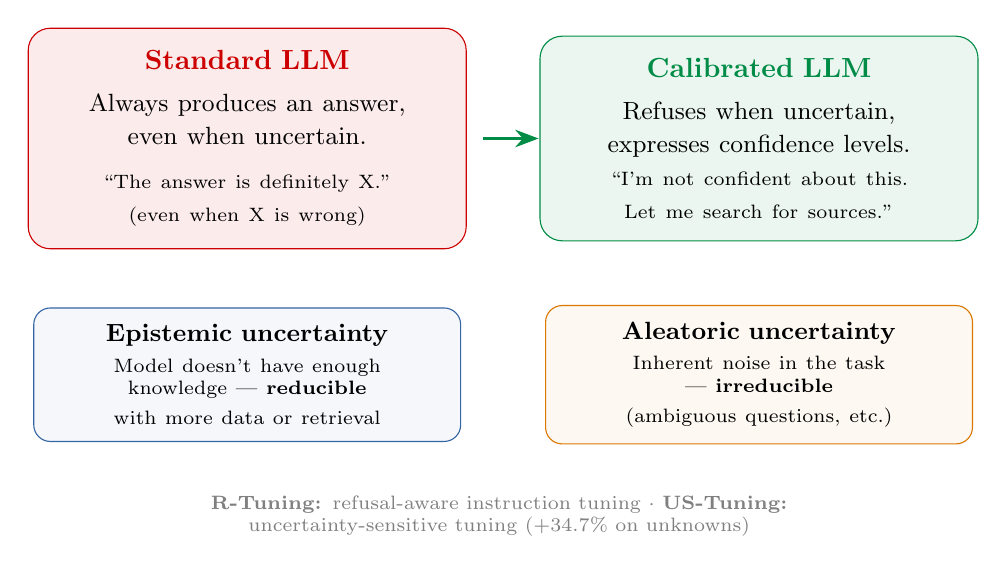
\begin{tikzpicture}
  % Standard vs calibrated
  \node[draw=sampred, fill=sampred!8, rounded corners=8pt, text width=5cm, align=center, inner sep=8pt] at (-3, 2) {
    \textbf{\textcolor{sampred}{Standard LLM}}\\[4pt]
    {\small Always produces an answer,\\even when uncertain.}\\[4pt]
    {\scriptsize ``The answer is definitely X.''}\\
    {\scriptsize (even when X is wrong)}
  };
  \node[draw=paramgreen, fill=paramgreen!8, rounded corners=8pt, text width=5cm, align=center, inner sep=8pt] at (3.5, 2) {
    \textbf{\textcolor{paramgreen}{Calibrated LLM}}\\[4pt]
    {\small Refuses when uncertain,\\expresses confidence levels.}\\[4pt]
    {\scriptsize ``I'm not confident about this.\\Let me search for sources.''}
  };

  \draw[-Stealth, very thick, paramgreen] (0, 2) -- (0.7, 2);

  % Types of uncertainty
  \node[draw=popblue, fill=popblue!5, rounded corners=6pt, text width=5cm, align=center, inner sep=6pt, font=\small] at (-3, -1) {
    \textbf{Epistemic uncertainty}\\[3pt]
    {\scriptsize Model doesn't have enough\\knowledge --- \textbf{reducible}\\with more data or retrieval}
  };
  \node[draw=orange1, fill=orange1!5, rounded corners=6pt, text width=5cm, align=center, inner sep=6pt, font=\small] at (3.5, -1) {
    \textbf{Aleatoric uncertainty}\\[3pt]
    {\scriptsize Inherent noise in the task\\--- \textbf{irreducible}\\(ambiguous questions, etc.)}
  };

  % Approaches
  \node[font=\scriptsize, text=gray, text width=11cm, align=center] at (0.2, -2.8) {
    \textbf{R-Tuning:} refusal-aware instruction tuning $\cdot$
    \textbf{US-Tuning:} uncertainty-sensitive tuning (+34.7\% on unknowns)
  };
\end{tikzpicture}
\end{center}
\end{frame}

% ============================================================
% MITIGATION LANDSCAPE
% ============================================================
\begin{frame}
\frametitle{The mitigation landscape}

\vspace{-0.3cm}
\begin{center}
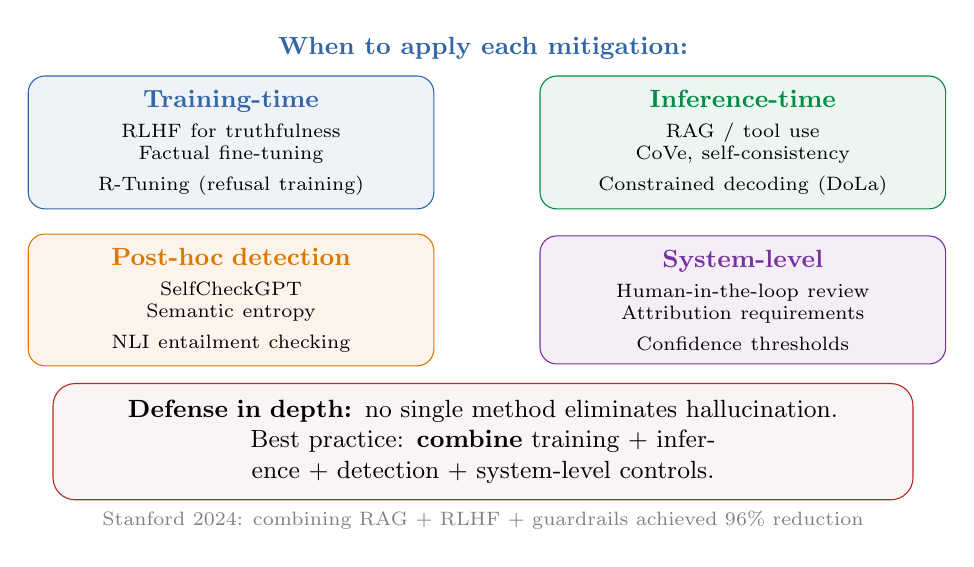
\begin{tikzpicture}
  % Title row
  \node[font=\small\bfseries, text=popblue] at (0, 3) {When to apply each mitigation:};

  % Training-time
  \node[draw=popblue, fill=popblue!8, rounded corners=6pt, text width=4.8cm, align=center, inner sep=5pt, font=\small] at (-3.2, 1.8) {
    \textbf{\textcolor{popblue}{Training-time}}\\[3pt]
    {\scriptsize RLHF for truthfulness\\Factual fine-tuning\\R-Tuning (refusal training)}
  };

  % Inference-time
  \node[draw=paramgreen, fill=paramgreen!8, rounded corners=6pt, text width=4.8cm, align=center, inner sep=5pt, font=\small] at (3.3, 1.8) {
    \textbf{\textcolor{paramgreen}{Inference-time}}\\[3pt]
    {\scriptsize RAG / tool use\\CoVe, self-consistency\\Constrained decoding (DoLa)}
  };

  % Post-hoc
  \node[draw=orange1, fill=orange1!8, rounded corners=6pt, text width=4.8cm, align=center, inner sep=5pt, font=\small] at (-3.2, -0.2) {
    \textbf{\textcolor{orange1}{Post-hoc detection}}\\[3pt]
    {\scriptsize SelfCheckGPT\\Semantic entropy\\NLI entailment checking}
  };

  % System-level
  \node[draw=violet1, fill=violet1!8, rounded corners=6pt, text width=4.8cm, align=center, inner sep=5pt, font=\small] at (3.3, -0.2) {
    \textbf{\textcolor{violet1}{System-level}}\\[3pt]
    {\scriptsize Human-in-the-loop review\\Attribution requirements\\Confidence thresholds}
  };

  % Defense in depth
  \node[draw=warnred, fill=warnred!5, rounded corners=8pt, text width=10.5cm, align=center, inner sep=6pt, font=\small] at (0, -2) {
    \textbf{Defense in depth:} no single method eliminates hallucination.\\
    Best practice: \textbf{combine} training + inference + detection + system-level controls.
  };

  \node[font=\scriptsize, text=gray] at (0, -3.0) {
    Stanford 2024: combining RAG + RLHF + guardrails achieved 96\% reduction
  };
\end{tikzpicture}
\end{center}
\end{frame}

% ============================================================
% PRACTICAL GUIDE
% ============================================================
\begin{frame}
\frametitle{Practical guide}

\begin{center}
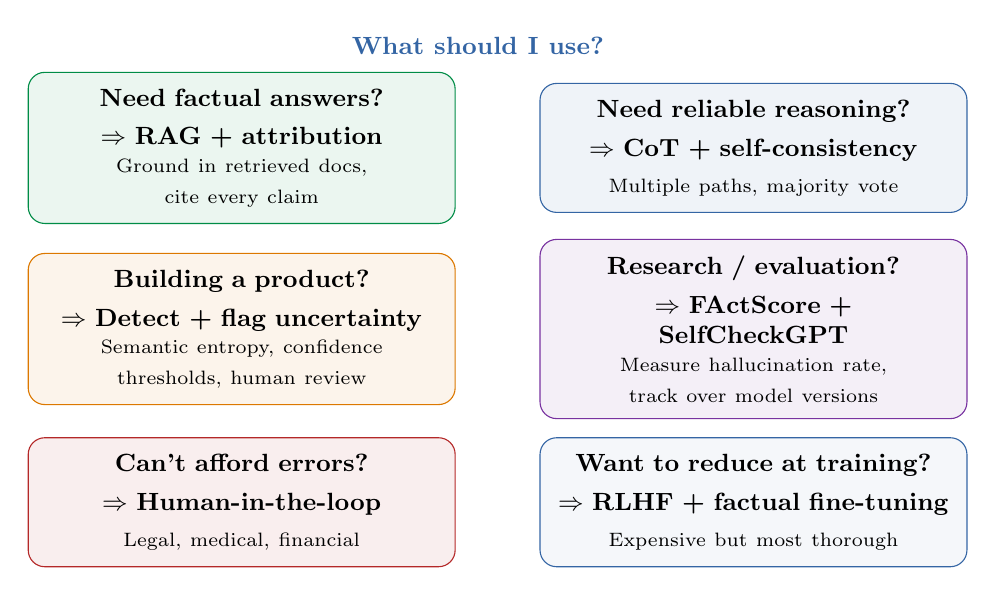
\begin{tikzpicture}
  \node[font=\small\bfseries, text=popblue] at (0, 3.3) {What should I use?};

  % Decision boxes
  \node[draw=paramgreen, fill=paramgreen!8, rounded corners=6pt, text width=5cm, align=center, inner sep=6pt, font=\small] at (-3, 2) {
    \textbf{Need factual answers?}\\[3pt]
    $\Rightarrow$ \textbf{RAG + attribution}\\[2pt]
    {\scriptsize Ground in retrieved docs,\\cite every claim}
  };
  \node[draw=popblue, fill=popblue!8, rounded corners=6pt, text width=5cm, align=center, inner sep=6pt, font=\small] at (3.5, 2) {
    \textbf{Need reliable reasoning?}\\[3pt]
    $\Rightarrow$ \textbf{CoT + self-consistency}\\[2pt]
    {\scriptsize Multiple paths, majority vote}
  };
  \node[draw=orange1, fill=orange1!8, rounded corners=6pt, text width=5cm, align=center, inner sep=6pt, font=\small] at (-3, -0.3) {
    \textbf{Building a product?}\\[3pt]
    $\Rightarrow$ \textbf{Detect + flag uncertainty}\\[2pt]
    {\scriptsize Semantic entropy, confidence\\thresholds, human review}
  };
  \node[draw=violet1, fill=violet1!8, rounded corners=6pt, text width=5cm, align=center, inner sep=6pt, font=\small] at (3.5, -0.3) {
    \textbf{Research / evaluation?}\\[3pt]
    $\Rightarrow$ \textbf{FActScore + SelfCheckGPT}\\[2pt]
    {\scriptsize Measure hallucination rate,\\track over model versions}
  };
  \node[draw=warnred, fill=warnred!8, rounded corners=6pt, text width=5cm, align=center, inner sep=6pt, font=\small] at (-3, -2.5) {
    \textbf{Can't afford errors?}\\[3pt]
    $\Rightarrow$ \textbf{Human-in-the-loop}\\[2pt]
    {\scriptsize Legal, medical, financial}
  };
  \node[draw=popblue, fill=popblue!5, rounded corners=6pt, text width=5cm, align=center, inner sep=6pt, font=\small] at (3.5, -2.5) {
    \textbf{Want to reduce at training?}\\[3pt]
    $\Rightarrow$ \textbf{RLHF + factual fine-tuning}\\[2pt]
    {\scriptsize Expensive but most thorough}
  };
\end{tikzpicture}
\end{center}
\end{frame}

% ============================================================
% QUESTIONS
% ============================================================
\begin{frame}
\begin{center}
\vspace{2cm}
{\Huge \textcolor{popblue}{Questions?}}

\vspace{1cm}
{\normalsize Next: Mixture of Experts}
\end{center}
\end{frame}

\end{document}
